\documentclass{beamer}
\usepackage[utf8]{inputenc}
\usepackage{graphics}
\mode<presentation> {
\usetheme{unc}}
\setbeamertemplate{navigation symbols}{} % To remove the navigation symbols from the bottom of all slides uncomment this line

\usepackage{graphicx} % Allows including images
\usepackage{booktabs} % Allows the use of \toprule, \midrule and \bottomrule in tables
\usepackage{media9} % Allows embedding of youtube videos


\usepackage{hyperref}
\hypersetup{linkcolor=blue,colorlinks=true}


% Remove symbols
\beamertemplatenavigationsymbolsempty


%\usetheme{default}

\usefonttheme{serif}

%----------------------------------------------------------------------------------------
%	TITLE PAGE
%----------------------------------------------------------------------------------------


\title[Global Challenges]{\LARGE{Global Challenges: Weapons of Mass Destruction and Climate Change}}
\author[POLI 150]{Steven Saroka}
\institute{POLI 150}
\date{30 April 2024}


\begin{document}

\begin{frame}
\titlepage % Print the title page as the first slide
\end{frame}


%----------------------------------------------------------------------------------------
%	PRESENTATION SLIDES
%----------------------------------------------------------------------------------------

\begin{frame} 
	\frametitle{\LARGE{Announcements}}
	\begin{itemize}
		\item Final Exam to be available from 12 AM on April 30 through 11:59 PM on May 3. Cumulative, 15-20 multiple choice questions, open-note and open-book, 2 hour 30 minute time limit.
		\item Prompts 12 and 13 due on April 30.
	\end{itemize}
\end{frame}

\begin{frame} 
	\frametitle{\LARGE{This Week's Class}}
	\begin{itemize}
		\item Weapons of Mass Destruction
			\begin{itemize}
			\item Defining WMD

			\item Nuclear deterrence

			\item Preventing nuclear proliferation 
			\end{itemize}
		\item Climate Change
			\begin{itemize}
			\item Patterns of international cooperation over climate change  
			
			\item Collective action problems review and application 
			
			\item Conflicts of interest in the environment 
		\end{itemize}
	\end{itemize}
\end{frame}


\begin{frame} 
	\frametitle{\LARGE{Key Terms}}
	\begin{itemize}
		\item WMD 
		\item MAD and mutual deterrence
		\item Non-Proliferation Treaty
		\item Coercive disarmament
		\item Climate change
		\item Common-pool resources
		\item Tragedy of the commons
		
	\end{itemize}
\end{frame}

\begin{frame} 
\frametitle{\LARGE{Central Question}}
\centering
	\Large{How should the world address the threat of global challenges, such as WMD and climate change?}
	
\end{frame}


\begin{frame} 
\frametitle{\LARGE{Weapons of Mass Destruction}}
\textbf{Weapons of Mass Destruction}: general term for weapons that can inflict damage on a massive scale. Three subcategories: \pause
\begin{itemize}
		\item \textbf{Chemical}: use of chemicals to kill or injure the enemy (e.g. mustard gas in WWI). \pause
		\item \textbf{Biological}: weaponized bacterium, virus, or other biological agents (e.g. anthrax in 2001). \pause
		\item \textbf{Nuclear}: explosive device that uses nuclear reactions (fission or fusion) (e.g. Hiroshima and Nagasaki).
\end{itemize}
\end{frame}

\begin{frame} 
	\frametitle{\LARGE{WMD Characteristics}}
What distinguishes a WMD from a conventional weapon? \pause
	\begin{itemize}
		\item \textbf{Indiscriminate violence}: these weapons cannot be precisely targeted. As such, they inflict violence not only on combatants but also on non-combatants in the area. \pause
		\item \textbf{Massive destructive potential}: such weapons enable destruction orders of magnitude above that accomplished by conventional weapons. \pause
		\item \textbf{Social norms}: to some extent, what is and is not a WMD is socially constructed.
	\end{itemize}
\end{frame}

\begin{frame} 
\frametitle{\LARGE{Chemical Weapons}}
\begin{itemize}
	\large{
		\item Modern use begins in WWI. \pause
		\item Over time, these have changed from simple containers of deadly gas to nearly undetectable nerve agents. \pause
		\item Used by states (Syrian government) and terrorist groups (Aum Shinrikyo in Tokyo in 1995). \pause 
		\item Chemical Weapons Convention (1997) outlaws production and stockpiling; 97\% of the worlds' stockpiles have been destroyed since then. 
		\item \href{https://www.opcw.org/}{Organization for the Prohibition of Chemical Weapons} is the organization implementing the CWC.
	}
\end{itemize}
\end{frame}

\begin{frame} 
\frametitle{\LARGE{Biological Weapons}}
\begin{itemize}
	\large{
		\item Used for centuries (e.g. smallpox blankets during French and Indian War, \href{https://www.history.com/news/colonists-native-americans-smallpox-blankets}{tthough it is unclear whether this worked}). \pause
		\item Developed further for use during the World Wars. \pause
		\item Used by states (Japan in WWII) and by terrorist groups (\href{https://en.wikipedia.org/wiki/1984_Rajneeshee_bioterror_attack}{1984 Oregon Salmonella attack}). \pause 
		\item Biological Weapons Convention (1972) bans use and stockpiling, but \href{https://www.armscontrol.org/factsheets/cbwprolif}{some states} maintain or are alleged to maintain an offensive capacity.
	}
\end{itemize}
\end{frame}

\begin{frame} 
\frametitle{\LARGE{Nuclear Weapons}}
\begin{itemize}
		\item Developed in the 1930s and 1940s. \pause
		\item Used twice in war (Hiroshima and Nagasaki). \pause
		\item Only possessed by nine countries. \pause 
		\item Non-Proliferation Treaty (1968) bans development and spread, but with mixed results.
\end{itemize}
\end{frame}

% Nuclear warheads image
 \begin{frame}{\LARGE Nuclear Powers 2020}
    \centering
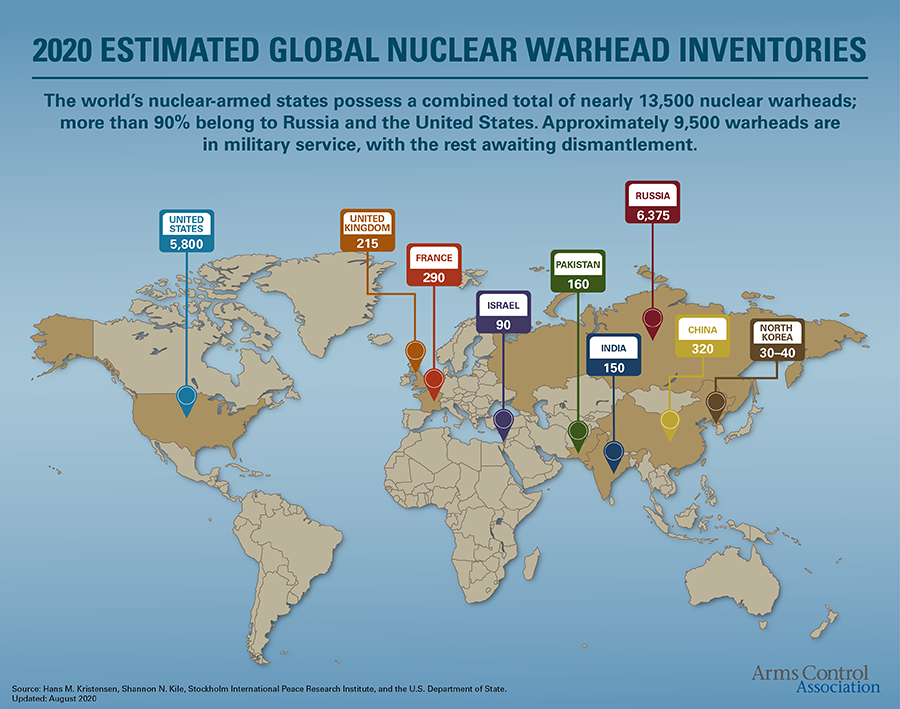
\includegraphics[width=\textwidth,height=0.9\textheight,keepaspectratio]{warheads.png}
\end{frame}

% Nuclear warheads image
\begin{frame}{\LARGE Nuclear Powers \href{https://www.sipri.org/media/press-release/2022/global-nuclear-arsenals-are-expected-grow-states-continue-modernize-new-sipri-yearbook-out-now}{2022}}
	\centering
	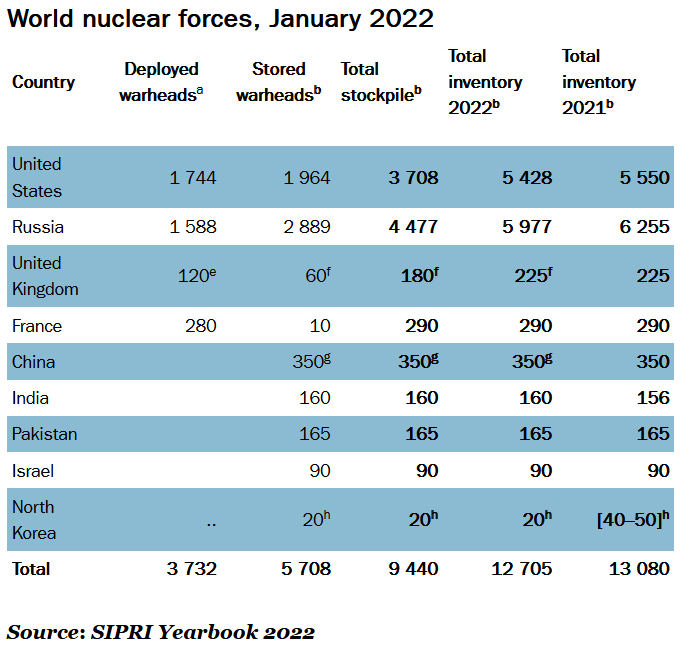
\includegraphics[width=\textwidth,height=0.9\textheight,keepaspectratio]{SIPRI2022nuclear.png}
\end{frame}

% Nuclear warheads image
\begin{frame}{\LARGE Nuclear Powers \href{https://www.sipri.org/media/press-release/2023/states-invest-nuclear-arsenals-geopolitical-relations-deteriorate-new-sipri-yearbook-out-now}{2023}}
	\centering
	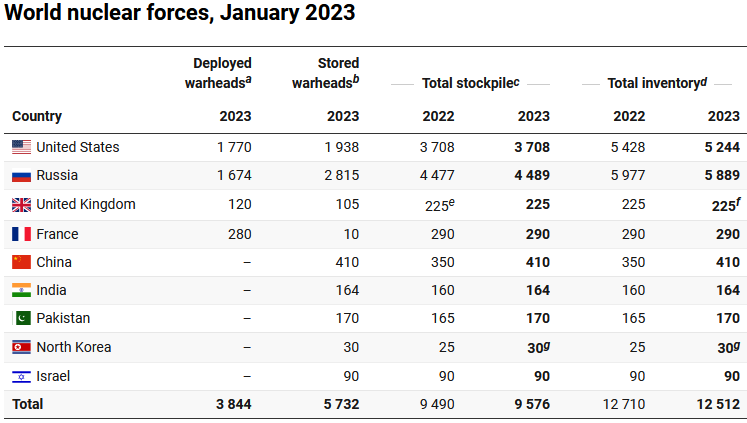
\includegraphics[width=\textwidth,height=0.9\textheight,keepaspectratio]{SIPRI2023nuclear.png}
\end{frame}

% Nuclear simulation 
\begin{frame}{\LARGE Modern-Day Nuclear Simulation 1}
    \centering
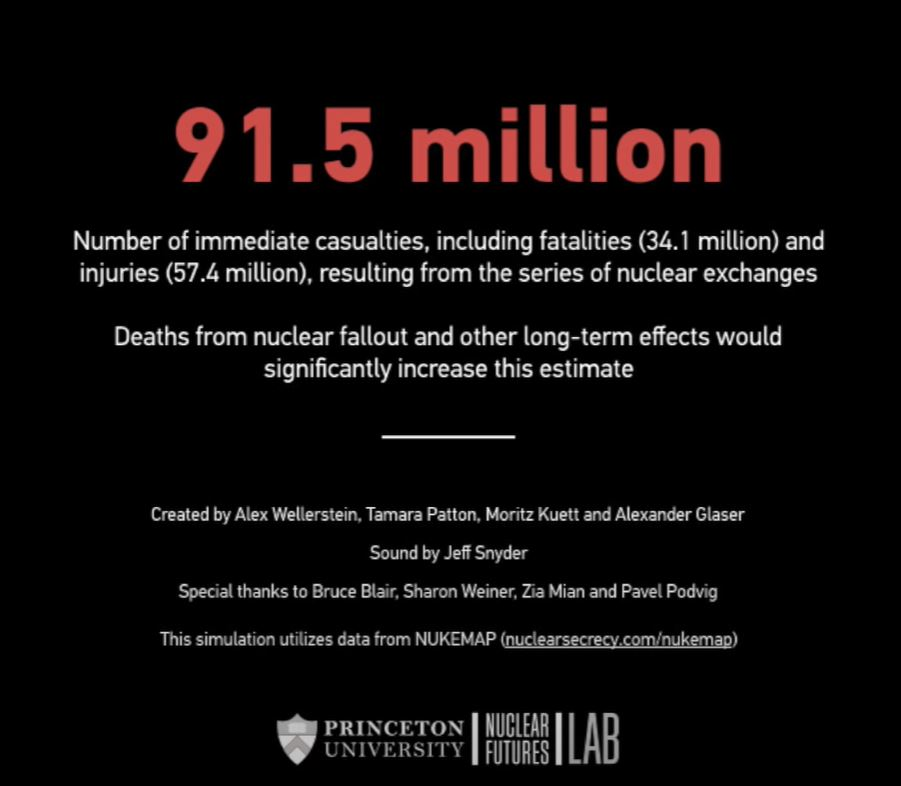
\includegraphics[width=\textwidth,height=0.9\textheight,keepaspectratio]{nuclear simulation.JPG}
\end{frame}

\begin{frame}{\LARGE Modern-Day Nuclear Simulation 2}
	\centering
	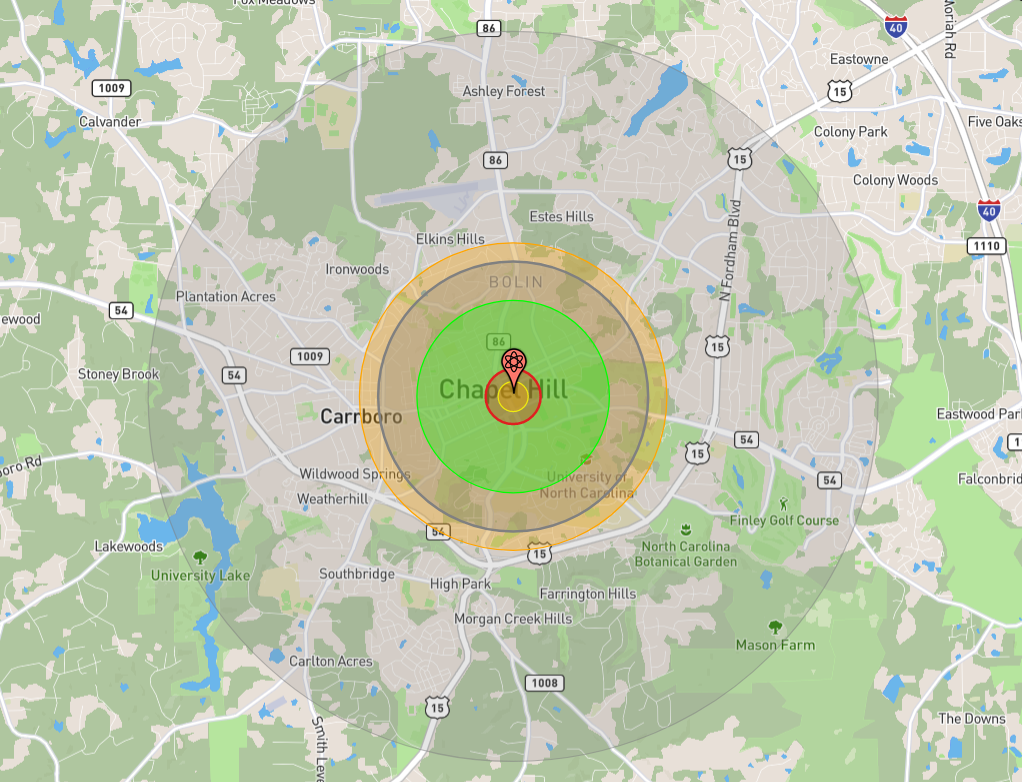
\includegraphics[width=\textwidth,height=0.9\textheight,keepaspectratio]{UNCnuke.png}
\end{frame}

\begin{frame} 
	\frametitle{\LARGE{Effects of Nuclear Weapons}}
	\begin{itemize}
		\item Prior slide shows impact of 15-kiloton bomb (same as used at Hiroshima) if dropped on our classroom. \href{https://nuclearsecrecy.com/nukemap/}{Source: Nukemap.} 
		\item Circle keys, from innermost: 	
		\begin{itemize}
			\item Fireball radius: instant death.
			\item Heavy blast damage radius: instant death.
			\item Radiation radius: fatalities from blast; fatal due to radiation in about a month.
			\item Moderate blast damage radius: Widespread building damage; high fatalities.
			\item Thermal radiation radius: Third-degree burns if exposed at this range.
			\item Light blast radius: survivable with moderate to minimal injuries (but probably affected by radiation).
		\end{itemize}
		\item Total deaths: at least 25,000. About 35,000 more injured.	
	\end{itemize}
\end{frame}

\begin{frame}{\LARGE Modern-Day Nuclear Simulation 3}
	\centering
	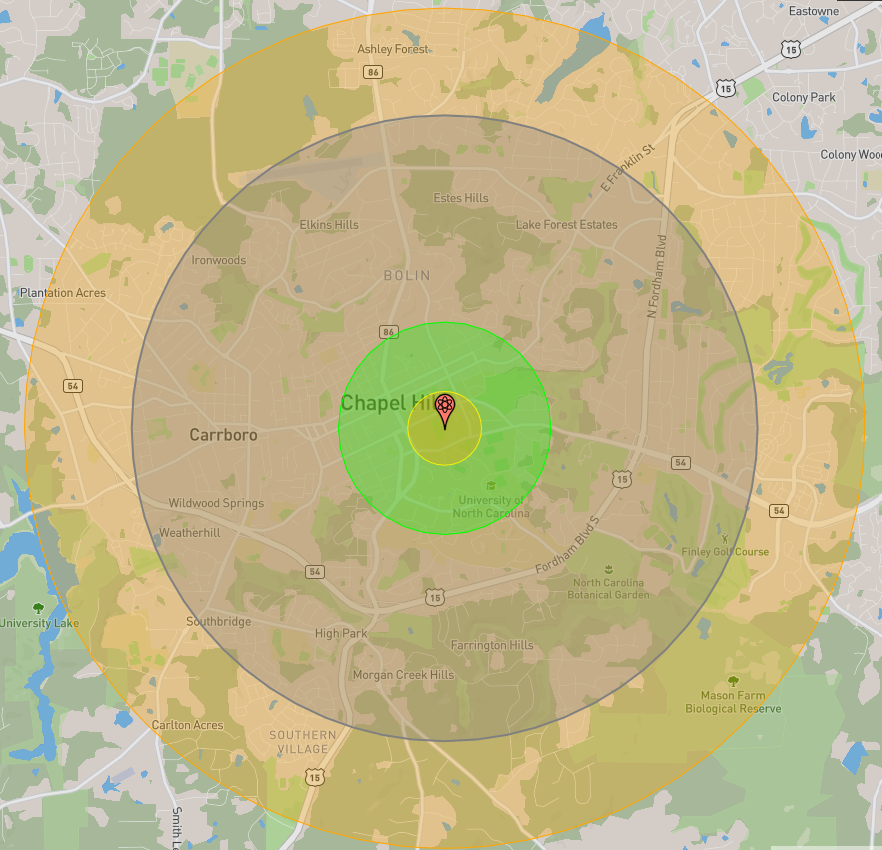
\includegraphics[width=\textwidth,height=0.9\textheight,keepaspectratio]{UNCnuke2.png}
\end{frame}

\begin{frame} 
\frametitle{\LARGE{Problems of WMD}}
\begin{itemize}
	\Large{
		\item (When) might WMD actually make war less likely? \pause
		\\~\\ 
		\item Why are states often unwilling to disarm? \pause
		\\~\\ 
		\item Why is monitoring of stockpiles and development so difficult? 
		\\~\\

	}
\end{itemize}
\end{frame}

\begin{frame} 
\frametitle{\LARGE{Nuclear Proliferation}}
\begin{itemize}

		\item Nuclear proliferation is often discussed as a massive problem facing the world. \pause
		\item Given the destructive capacity of nuclear weapons, many argue that the international community may be safer without them. \pause
		\item However, it is possible to argue that nuclear proliferation is a force for peace and stability...
	
\end{itemize}
\end{frame}

\begin{frame} 
\frametitle{\LARGE{Theoretical Considerations}}
\begin{itemize}

		\item A realist perspective, treating state actors as rational and focused on survival, makes nuclear war unappealing. \pause
		\item Nuclear war is arguably the worst possible outcome for a state. \pause
		\item In the language of the bargaining model of war, nuclear weapons mean that the costs $c$ become essentially infinite, removing any possibility of gains from war.
		\item Mutually assured destruction is one proposed solution to this.
	
\end{itemize}
\end{frame}

\begin{frame} 
	\frametitle{\LARGE{Mutually Assured Destruction (MAD)}}
	\begin{itemize}
	\item \textbf{Mutually Assured Destruction}: guaranteed destruction if two nuclear-armed adversaries use their nuclear weapons on each other. \pause
	\item MAD should create an environment of \textbf{mutual deterrence}: neither side will attack the other, forcing them to find other means of resolving disputes.
	\end{itemize}
\end{frame}

\begin{frame} 
\frametitle{\LARGE{Mutual Deterrence Requirements}}
Requirements for MAD to work: \pause
\begin{enumerate}
		\item Each state has \textbf{second-strike capabilities}. \pause
		\item Leaders care about their survival. \pause
		\item Weapons not be easily subject to accidental launch. \pause
		\item Easy to determine origins of any given attack.
\end{enumerate}
\end{frame}

\begin{frame} 
\frametitle{\LARGE{Nuclear Concerns}}
Given the successful track-record of deterrence thus far, why do we care about nuclear proliferation (as well as WMD proliferation in general)? \pause
	\begin{itemize}
		\item Even if they reduce the probability of nuclear war, nuclear weapons influence the distribution of power. \pause
		\item There is a risk of nonstate actors gaining possession (especially for non-nuclear WMD). \pause 
        \item Some states may not meet the requirements for effective MAD deterrence. \pause 		
        \item \textbf{Mistakes happen!}
\end{itemize}
\end{frame}

\begin{frame} 
	\frametitle{\LARGE{Goldsboro, NC Accident}}
	\begin{figure}
		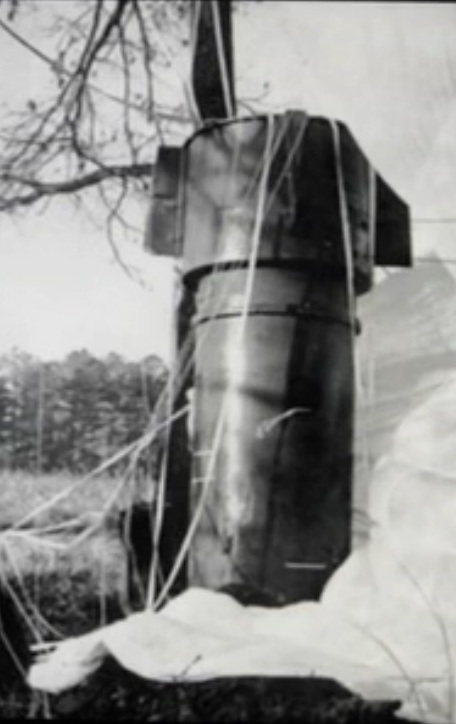
\includegraphics[height=.85\textheight,keepaspectratio]{./goldsboro.jpg}
	\end{figure}
\end{frame}

\begin{frame} 
\frametitle{\LARGE{Goldsboro, NC Nuclear Accident}}
\begin{itemize}
	\item On January 23, 1961, an American B-52 Stratofortress flying over NC broke apart due to structural failure. \pause
	\item It was carrying two 3-4 megaton bombs, both of which fell free of the aircraft during the crash. \pause
	\item One bomb's parachute deployed, and it landed safely. \pause
	\item The other one was armed, with a single switch between it and the possibility of detonation. \pause
	\item This isn't even the only nuclear accident involving US nuclear weapons (\href{https://en.wikipedia.org/wiki/List_of_military_nuclear_accidents}{list}).
	\item USSR \href{https://en.wikipedia.org/wiki/1983_Soviet_nuclear_false_alarm_incident}{also made mistakes.}
\end{itemize}
\end{frame}

\begin{frame} 
	\frametitle{\LARGE{Goldsboro Accident Bomb Size}}
	\begin{figure}
		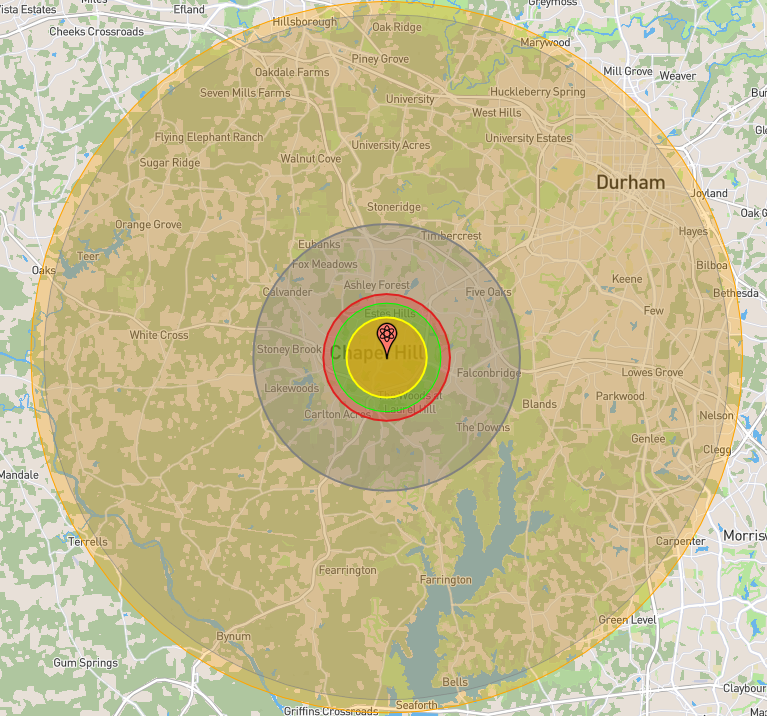
\includegraphics[width=\textwidth,height=0.9\textheight,keepaspectratio]{1961accidentsize.png}
	\end{figure}
\end{frame}

\begin{frame} 
\frametitle{\LARGE{Preventing Nuclear Proliferation}}
With these concerns in mind, states and some NGOs have attempted to prevent nuclear proliferation in two ways: \pause
\begin{enumerate}
	\item Altering incentives
	\item Preventing actors from accessing nuclear materials
\end{enumerate}
\end{frame}

\begin{frame} 
\frametitle{\LARGE{Altering Nuclear Incentives}}
 What interest does a state have in acquiring nuclear weapons? \pause 
\begin{itemize}
		\item States attempt to acquire nuclear weapons out of insecurity due to anarchy. \pause
		\item This implies that guaranteeing their security can prevent them from seeking weapons of their own.
\end{itemize}
\end{frame}

\begin{frame} 
\frametitle{\LARGE{Altering Nuclear Incentives}}
\begin{itemize}
		\item Credible nuclear defensive alliances are one way to guarantee security for a state without that state having to acquire nuclear weapons of its own. \pause
		\item Successful example: NATO. Less successful example: Ukraine.
\end{itemize}
\end{frame}

\begin{frame}{\LARGE Nuclear Umbrella}
    \centering
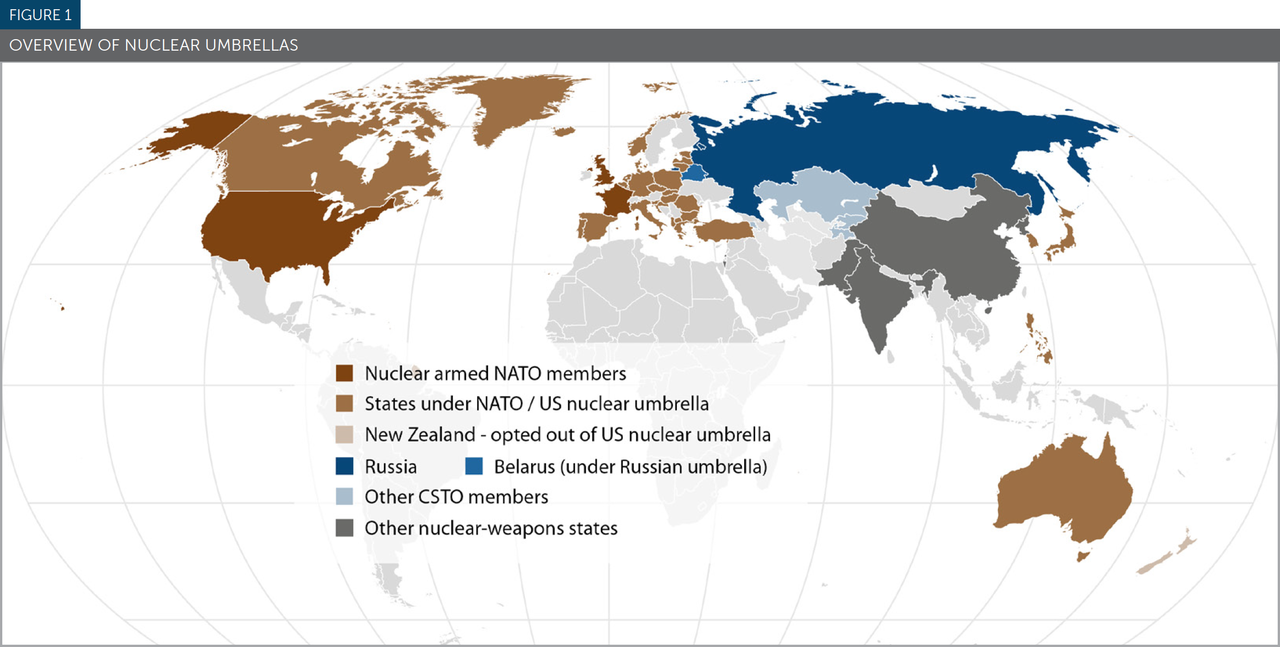
\includegraphics[width=\textwidth,height=0.8\textheight,keepaspectratio]{nuclear umbrella.png}
\end{frame}

\begin{frame} 
	\frametitle{\LARGE{Preventing Access}}
	\begin{itemize}
		\item \textbf{Coercive disarmament:} threatening or using military force to disrupt or prevent nuclear development (ex: Israeli efforts against Iran). 
		\begin{itemize}
			\item Examples of access prevention campaigns include North Korea (ultimately acquired nuclear weapons) and Iran (ongoing). \pause
		\end{itemize}
		\item States may also create monitoring and tracking efforts to prevent nuclear material and information from going to either rogue states or non-state actors, sometimes supported by international agreements such as the nuclear \textbf{Non-Proliferation Treaty (NPT)}.
	\end{itemize}
\end{frame}

\begin{frame} 
\frametitle{\LARGE{Iran's Nuclear Program}}
\begin{itemize}
		\item Iran has actively pursued nuclear research for both energy and weapons. \pause
		\item It has faced harsh international sanctions for its efforts. \pause
		\item It has also faced sabotage (ex: Stuxnet) and targeted assassination against its nuclear program. 
		\item In 2015, a deal (the JCPOA) was reached to lift sanctions in exchange for a large scale reduction in its nuclear program. \pause
		\begin{itemize}
			\item JCPOA parties: US, Iran, other P5 members, Germany, other EU members \pause
		\end{itemize}
		\item US withdrew from the JCPOA in 2018, effectively killing it; Iranian progress towards nuclear weapons has since resumed.
\end{itemize}
\end{frame}

\begin{frame} 
\frametitle{\LARGE{Assessing the NPT}}
\begin{itemize}
		\item The \textbf{Non-Proliferation Treaty} prohibits all states except for the original five nuclear states from having nuclear weapons. \pause
		\item Provides for monitoring of compliance through the International Atomic Energy Agency. \pause 
		\item The IAEA can submit charges to the UNSC, asking it to impose sanctions. \pause
		\item Has had successes (South Africa, Brazil, Argentina) and weaknesses (North Korea, Iraq, Iran, Libya, Ukraine). \pause
		\item Has the NPT been successful? Somewhat.
\end{itemize}
\end{frame}



\begin{frame} 
\frametitle{\LARGE{The Global Zero Movement}}
\begin{itemize}
		\item (Relatively) informal efforts to reduce nuclear weapons have also emerged. \pause \item One example is \href{https://www.globalzero.org/}{Global Zero}: network of political leaders, activists, military officials, and civic leaders advocating for 0 nuclear weapons. \pause
		\item Public opinion generally favors reduction of nuclear weapons. \pause 
		\item Is this possible? Desirable? \pause 
		\item Can the US credibly lead a disarmament movement? 
\end{itemize}
\end{frame}


\begin{frame} 
\frametitle{\LARGE{To Ponder...}}
\centering
	\Large{Is the world safer with or without nuclear weapons? \\~\\ What would it take to get to a world without nuclear weapons?}
	
\end{frame}

\begin{frame} 
	\frametitle{\LARGE{Climate Change Definitions}}
	\begin{itemize}
		\item \textbf{Climate change AKA ``global warming"}: human-induced environmental changes leading to increased global temperatures and shifting weather patterns. \pause
		\item This is distinct from (and more extreme than) the natural changes to Earth's climate (e.g. start and end of ice ages).
		\item ``Scientific evidence for warming of the climate system is unequivocal." - UN's Intergovernmental Panel on Climate Change (\href{https://www.ipcc.ch/}{IPCC site})
		\item See \href{https://climate.nasa.gov/evidence/}{NASA} for more details and evidence.
	\end{itemize}
\end{frame}

%https://climate.nasa.gov/evidence/
\begin{frame} 
	\frametitle{\LARGE{Atmospheric CO2}}
	\begin{figure}[ht!]
		\centering
		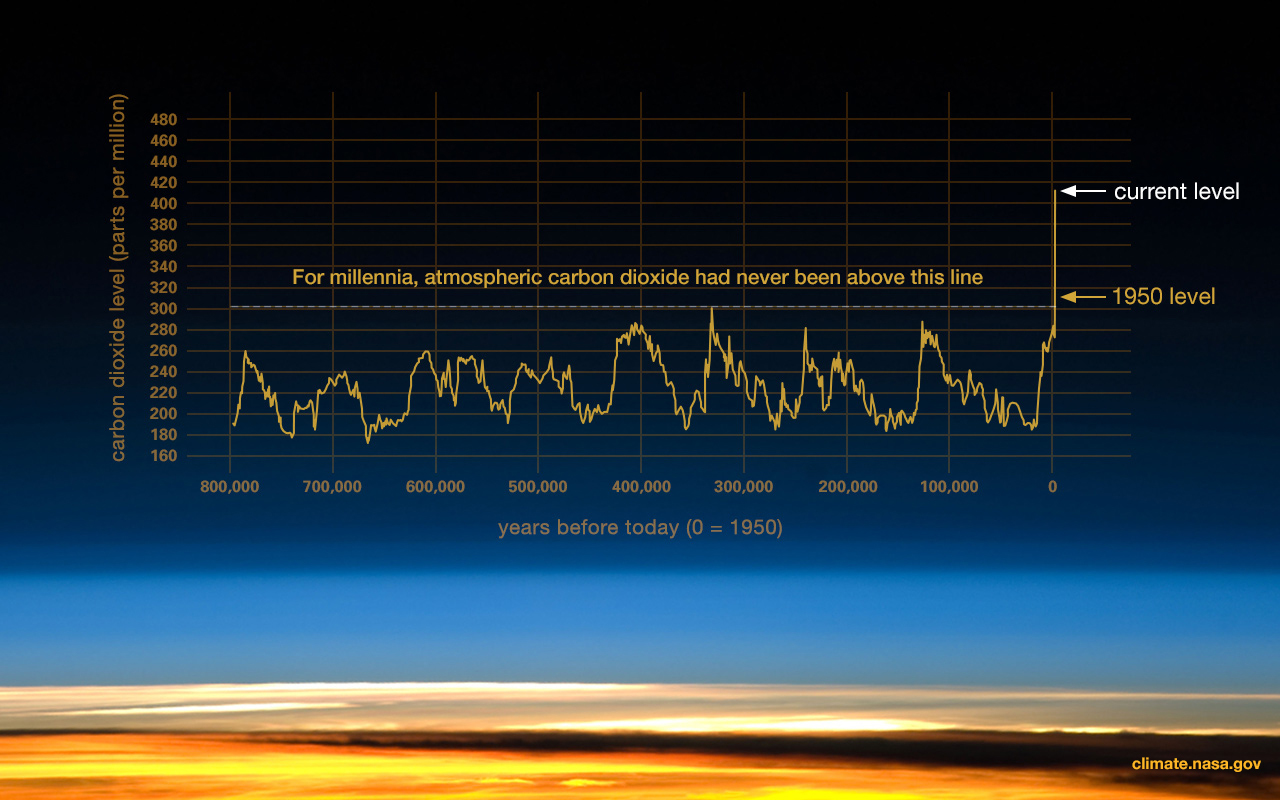
\includegraphics[width=\textwidth,height=0.9\textheight, keepaspectratio]{NASAco2.jpg}
	\end{figure}
\end{frame}

\begin{frame} 
	\frametitle{\LARGE{Arctic Sea Ice Shrinkage}}
	\begin{figure}[ht!]
		\centering
		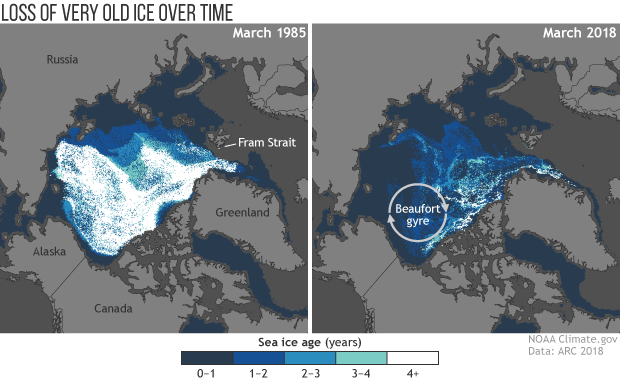
\includegraphics[width=\textwidth,height=0.8\textheight, keepaspectratio]{arctic_sea_ice.png}
	\end{figure}
\end{frame}

\begin{frame} 
	\frametitle{\LARGE{Antarctic Ice Shrinkage}}
	\begin{figure}[ht!]
		\centering
		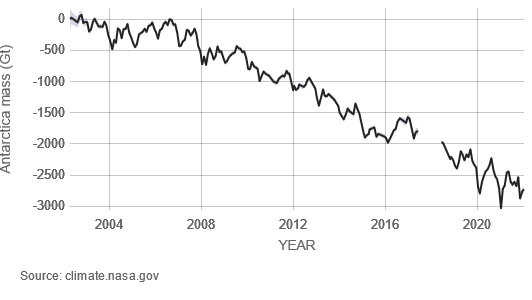
\includegraphics[width=\textwidth,height=0.8\textheight,keepaspectratio]{LandIceAntarctica.png}
	\end{figure}
\end{frame}

\begin{frame} 
	\frametitle{\LARGE{Politically Salient Impacts}}
	List drawn partially from \href{https://climate.nasa.gov/evidence/}{NASA}.
	\begin{itemize}
		\item Rising temperatures and melting ice means rising sea levels. This threatens low-lying coastal areas; existential threat to island states. \pause
		\item Warming ocean threatens to disrupt oceanic ecosystems, indirectly threatening fishing and related industries. \pause
		\item Increased disruption of weather patterns and increased incidence of extreme weather events (wildfire, hurricanes, etc.), leading to economic damage and disruption.
		\item Weather changes also disrupt agricultural patterns (esp. in poorer, warmer countries). \pause
		\item IR experts believe these effects of climate change will make conflict more likely (\href{https://www.un.org/peacebuilding/fr/news/climate-change-recognized-\%E2\%80\%98threat-multiplier\%E2\%80\%99-un-security-council-debates-its-impact-peace}{UNSC}). 
	\end{itemize}
\end{frame}

\begin{frame} 
	\frametitle{\LARGE{Climate Change and Conflict}}
	\begin{figure}[ht!]
		\centering
		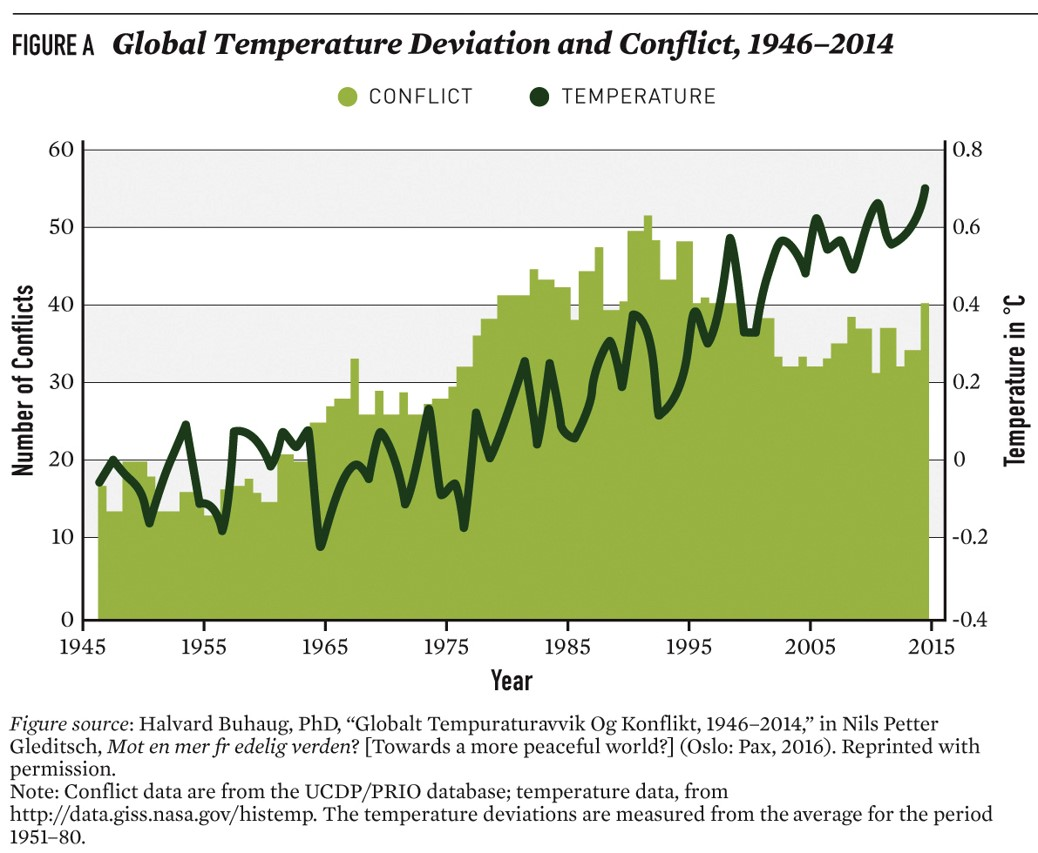
\includegraphics[width=\textwidth,height=0.9\textheight, keepaspectratio]{conflict.jpg}
	\end{figure}
\end{frame}

\begin{frame} 
	\frametitle{\LARGE{International Cooperation}}
	Governments have made some progress in cooperating to combat climate change.
	\begin{itemize}
		
		\item \textbf{Montreal Protocol (1987)}: phased out consumption and production of ozone-depleting substances, with evidence of ozone layer repairing itself. \pause 
		
		\item \textbf{United Nations Framework Convention on Climate Change (UNFCCC) (1992)}: soft law that provides structure for efforts on climate change. \pause
		
		\item \textbf{Kyoto Protocol (1997)}: established specific targets for reducing greenhouse gas emissions. \pause
		
		\item \textbf{Paris Agreement (2016)}: commitments from 196 countries to reduce emissions.
		
	\end{itemize}
\end{frame}

\begin{frame} 
	\frametitle{\LARGE{Obstacles to Effective Cooperation}}
	\begin{itemize}
		\item Despite these agreements, cooperation over climate policy has failed to reverse the trends of climate change. \pause
		
		\item Problem: Individual actors might have interests in improving the environment, but individual action has little effect. \pause
		
		\item Example: 15-20 countries account for 75\% of carbon dioxide emissions, but not a single country accounts for more than 30\%. \pause 
		
		\item This phenomenon relating to global cooperation over the environment is often likened to the \textbf{Tragedy of the Commons}.
		
	\end{itemize}
\end{frame}

\begin{frame} 
	\frametitle{\LARGE{Tragedy of the Commons Definition}}
	\begin{itemize}
		\item If a resource is open to all without limit, no one individual has an incentive to conserve that resource. \pause
		
		\item As a result, the resource degrades over time until it is completely depleted/unusable. \pause 
		\item \textbf{Crucially, no single individual's actions can solve the problem.} \pause 
		
		\item Examples: \pause fisheries, forests, global atmosphere, livable planet \pause
		
		\item The tragedy of the commons explains why states struggle to maintain global \textbf{public goods}.
	\end{itemize}
\end{frame}

\begin{frame} 
	\frametitle{\LARGE{Types of Goods}}
	Goods differ on two axes: rivalry and excludability.
	\begin{itemize}
		
		\item Excludable: action can be selectively (not) allowed to use a good. \pause
		
		\item Rivalrous: consumption by one actors reduces the amount available for others to consume. 
	\end{itemize}
\end{frame}

\begin{frame} 
	\frametitle{\LARGE{Types of Goods}}
	\begin{figure}[ht!]
		\centering
		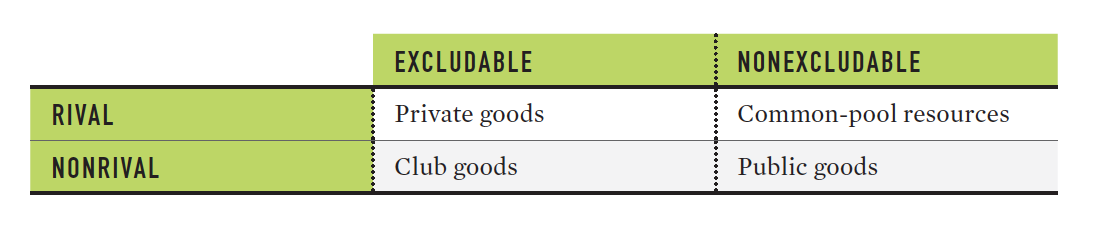
\includegraphics[width=\textwidth,height=0.8\textheight, keepaspectratio]{./goods.png}
	\end{figure}
\end{frame}

\begin{frame} 
	\frametitle{\LARGE{Climate and Collective Action}}
	\begin{itemize}
		\item \textbf{The tragedy of the commons is not the same as a collective action problem.} \pause
		\item Recall the definition of a \textbf{collective action problem}: all members of a group benefit from the provision of the public good, but all have incentives to ``defect" by not helping pay the costs of providing the good, and so the public good is never provided. \pause
		\item In a CAP, actors must work together to provide the good. In a TOC the good exists already and actors must coordinate on its use.
	\end{itemize}
\end{frame}



\begin{frame} 
	\frametitle{\LARGE{Climate and Collective Action}}
	\begin{itemize}
		\large{
			\item The benefits of a stable global climate are generally a mixture of public goods and common-pool resources. \pause
			
			\item Common-pool resources fall victim to the tragedy of the commons. \pause
			
			\item Public goods are subject to collective action problems. \pause 
			
			\item Rational actors have (short-term) incentives to engage in self-interested behavior that ultimately has negative impacts on both public goods and common-pool resources.
		}
	\end{itemize}
\end{frame}

\begin{frame} 
	\frametitle{\LARGE{Complicating Factors}}
	Several factors make CAPs and TOCs harder to solve. \pause
	\begin{itemize}
		\item \textbf{Size}: more members make CAPs harder to solve (acid rain vs. atmosphere). \pause
		
		\item \textbf{Complexity}: more complex problems are harder to solve (``dirty-dozen'' chemicals). \pause
		
		\item \textbf{Iteration and linkage}: interacting repeatedly can solve CAP (but this works better with limited number of actors). \pause 
		
		\item \textbf{Bundling}: tying private gains to public goods (advantages of forests). \pause 
		
		\item \textbf{Intensity Disparity}: more affected parties are more likely to bear costs of solutions, if they can.
		
	\end{itemize}
\end{frame}

\begin{frame} 
	\frametitle{\LARGE{Success Story: Montreal Protocol}}
	\begin{itemize}
		\large{
			\item Signed in 1980s to address production and consumption of ozone-depleting substances \pause
			
			\item Size: limited number of participants, but large enough to matter. \pause
			
			\item Bundling: trade restrictions to enforce participation. \pause
			
			\item Complexity: scientifically relatively easy to determine a threshold of success.
		}
	\end{itemize}
\end{frame}

\begin{frame} 
	\frametitle{\LARGE{Future Success? The Paris Agreement}}
	\begin{itemize}
		\large{
			\item Signed in 2016, it is \textit{the} major environment agreement. \pause
			
			\item Size: nearly every country of importance. \pause
			
			\item Complexity: no clear threshold beyond goal of limiting global temperature increase to +2 Celsius over pre-industrial levels, via reducing greenhouse gas emissions. \pause 
			
			\item Bundling: none (countries choose their own emissions and schedules). \pause 
			
			\item US left under Trump then rejoined under Biden, but the framework may be of limited viability if it becomes a revolving door...
			
		}
	\end{itemize}
\end{frame}


\begin{frame} 
	\frametitle{\LARGE{Taxation as a Solution?}}
	\begin{itemize}
		\large{\pause
			\item Economists have suggested taxing carbon emissions. \pause
			
			\item Makes the cost of using carbon fuels reflect the costs to society for continued usage. \pause
			
			\item Problem? \pause Extremely unpopular with industries and consumers! \pause
			\item Additional problem: this does not necessarily eliminate emissions!
		}
	\end{itemize}
\end{frame}

\begin{frame} 
	\frametitle{\LARGE{`Property Rights' as a Solution?}}
	\begin{itemize}
		\large{
			\item An alternative solution focuses on rights to emit. \pause
			
			\item Some places like Europe or California use a cap-and-trade system. \pause
			
			\item Firms are allotted a set level of emissions, and can buy and sell ``credits'' if they fall below or above the thresholds. \pause
			
			\item Creates an incentive to develop green technologies.
		}
	\end{itemize}
\end{frame}

\begin{frame} 
	\frametitle{\LARGE{Industry Pressures}}
	\begin{itemize}
		\large{
			\item Firms and industries have interests in opposing environmental policies that restrict their profitability. \pause
			
			\item Increased environmental constraints would force them to expend more (e.g. treating waste). \pause
			
			\item Green energy increases competition for traditional energy industries. \pause
			
			\item Consumers also benefit from lax environmental policies, as prices are lower. \pause 
			
			\item Thus, much like the politics of trade, environmental regulations produces winners and losers, which structures domestic political interactions.
		}
	\end{itemize}
\end{frame}

\begin{frame} 
	\frametitle{\LARGE{Bottom-Up Pressure}}
	\begin{itemize}
		\large{
			\item There are more individuals that would benefit from a green environment than a degraded environment. \pause
			
			\item Why don't we see more green policies? \pause Firms' interests are better organized, and are better able to press the government for lax policies. \pause
			
			\item Very similar to protectionist industries' influence over trade policy. \pause
			
			\item Furthermore, some firms \textit{benefit} from climate change (e.g. Exxon-Mobil and Arctic oil deposits). 
			
		}
	\end{itemize}
\end{frame}

\begin{frame} 
	\frametitle{\LARGE{International Variation in Emission}}
	\begin{figure}[ht!]
		\centering
		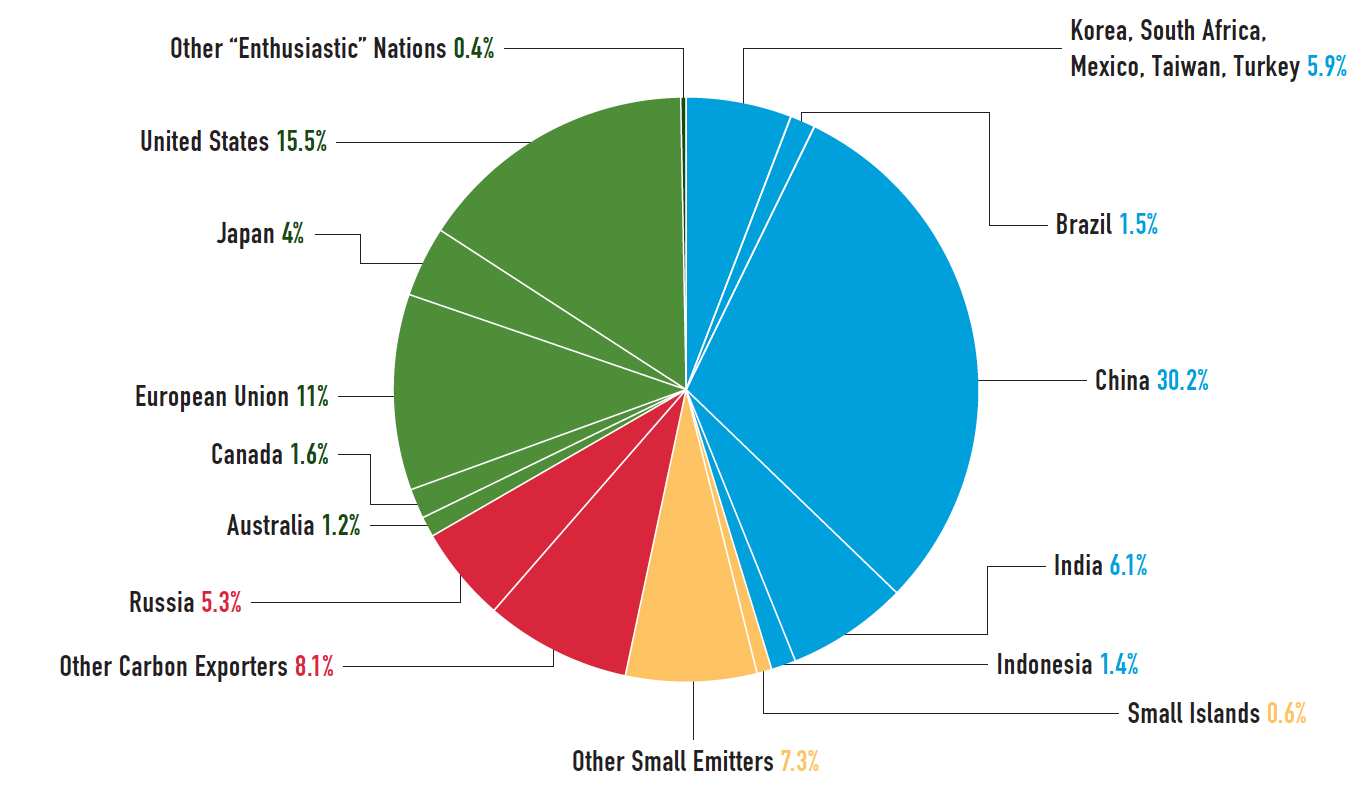
\includegraphics[width=\textwidth,height=0.8\textheight, keepaspectratio]{./emit_dist.png}
	\end{figure}
\end{frame}

\begin{frame} 
	\frametitle{\LARGE{Developed vs. Developing Countries}}
	\begin{itemize}
		\large{
			\item Historically, developed countries have been most egregious polluters. \pause
			
			\item Most states increase their pollution as they develop until they hit a threshold of relatively high development, then become interested in controlling pollution. \pause
			
			\item In the future, increases in emission will come from today's developing countries. \pause
			
			\item Globally, there are incentives to enact environmentalist policies; at the state level, these developing states may disagree if such policies limit their development.
		}
	\end{itemize}
\end{frame}

\begin{frame} 
	\frametitle{\LARGE{Summary}}
	\begin{itemize}
		\item Climate change is expected to have serious environmental and political impacts in the coming decades. \pause
		\item Addressing climate change requires states solve a mixture of collective action problems and tragedies of the commons. \pause
		\item These efforts are complicated by the size and complexity of the issues. \pause
		\item Substantial competing interests: LDCs vs. developed states, industries vs. citizens, etc. \pause
		\item Some international treaties provide cause for hope?		
	\end{itemize}
\end{frame}

\end{document}
